\documentclass[ignorenonframetext,]{beamer}

\setbeamertemplate{caption}[numbered]
\setbeamertemplate{caption label separator}{: }
\setbeamercolor{caption name}{fg=normal text.fg}

\beamertemplatenavigationsymbolsempty
\usepackage{lmodern}
\usepackage{amssymb,amsmath}
\usepackage{ifxetex,ifluatex}
\usepackage{fixltx2e} % provides \textsubscript
\ifnum 0\ifxetex 1\fi\ifluatex 1\fi=0 % if pdftex
  \usepackage[T1]{fontenc}
  \usepackage[utf8]{inputenc}
\else % if luatex or xelatex
  \ifxetex
    \usepackage{mathspec}
  \else
    \usepackage{fontspec}
  \fi
  \defaultfontfeatures{Ligatures=TeX,Scale=MatchLowercase}
\fi

% Start adding some content
\usepackage{graphicx}
\usepackage{color}
\usepackage{beamerthemebars}
\usepackage{multicol}
\usepackage{multirow}
\usepackage{hyperref}


\usetheme{Frankfurt}
%%redefined colors for beamer
%\definecolor{beamer@UIUCblue}{RGB}{0,60,125}
%\definecolor{beamer@UIUCorange}{RGB}{244,127,36}
%% taken from
%% http://identitystandards.illinois.edu/graphicstandardsmanual/generalguidelines/colors.html
%
%\definecolor{beamer@UIUCgray}{RGB}{210,210,210}
%\definecolor{beamer@UIUCgray2}{RGB}{244,244,244}
%
%\setbeamercolor{frametitle}{fg=beamer@UIUCblue,bg=beamer@UIUCgray}
%\setbeamercolor{normal text}{fg=black}
%\setbeamercolor{title}{fg=beamer@UIUCblue,bg=beamer@UIUCorange}
%\setbeamercolor{item projected}{fg=white,bg=beamer@UIUCorange}
%
%% Boxes
%\setbeamercolor{block title}{fg=beamer@UIUCblue,bg=beamer@UIUCorange}
%\setbeamercolor{block body}{fg=blue,bg=beamer@UIUCblue!80}
%\setbeamercolor{title in head/foot}{fg=beamer@UIUCblue,bg=beamer@UIUCgray}
%\setbeamercolor{author in head/foot}{fg=white,bg=beamer@UIUCblue}
%\setbeamercolor{institute in head/foot}{fg=white,bg=beamer@UIUCorange}
%\setbeamercolor{date in head/foot}{fg=white,bg=beamer@UIUCorange}
%\setbeamercolor{section in head/foot}{fg=white,bg=beamer@UIUCblue}
%\setbeamercolor{subsection in head/foot}{fg=white,bg=beamer@UIUCorange}
%
%
%\hypersetup{colorlinks=true,urlcolor=beamer@UIUCblue,linkcolor=beamer@UIUCblue,% link color controls section, subsection, and title
%citecolor = beamer@UIUCorange,
%anchorcolor = beamer@UIUCorange}
%
%%override title link color
%\addtobeamertemplate{headline}{\hypersetup{linkcolor=.}}{}
%\addtobeamertemplate{footline}{\hypersetup{linkcolor=.}}{}
%
%% Setup blocks
%\setbeamercolor{block title}{fg = white, bg = beamer@UIUCblue}
%\setbeamercolor{block body}{fg=black,bg=beamer@UIUCgray2}
%
%\setbeamercolor{block title alerted}{fg = white, bg = beamer@UIUCorange}
%\setbeamercolor{block body alerted}{fg=black,bg=beamer@UIUCgray2}
%
%\setbeamercolor{block title example}{fg = beamer@UIUCblue, bg = beamer@UIUCgray}
%\setbeamercolor{block body example}{fg=black,bg=beamer@UIUCgray2}

% use upquote if available, for straight quotes in verbatim environments
\IfFileExists{upquote.sty}{\usepackage{upquote}}{}
% use microtype if available
\IfFileExists{microtype.sty}{%
\usepackage{microtype}
\UseMicrotypeSet[protrusion]{basicmath} % disable protrusion for tt fonts
}{}
\newif\ifbibliography
\usepackage{graphicx,grffile}
\makeatletter
\def\maxwidth{\ifdim\Gin@nat@width>\linewidth\linewidth\else\Gin@nat@width\fi}
\def\maxheight{\ifdim\Gin@nat@height>\textheight0.8\textheight\else\Gin@nat@height\fi}
\makeatother
% Scale images if necessary, so that they will not overflow the page
% margins by default, and it is still possible to overwrite the defaults
% using explicit options in \includegraphics[width, height, ...]{}
\setkeys{Gin}{width=\maxwidth,height=\maxheight,keepaspectratio}

% Prevent slide breaks in the middle of a paragraph:
\widowpenalties 1 10000
\raggedbottom

\AtBeginSection[]
{
  \ifbibliography
  \else
    \let\insertsectionnumber\relax
    \let\sectionname\relax
    \begin{frame}
      \frametitle{On the Agenda}
      \begin{multicols}{2}
      \tableofcontents[currentsection]
      \end{multicols}
    \end{frame}
  \fi
}

\setlength{\parindent}{0pt}
\setlength{\parskip}{6pt plus 2pt minus 1pt}
\setlength{\emergencystretch}{3em}  % prevent overfull lines
\providecommand{\tightlist}{%
  \setlength{\itemsep}{0pt}\setlength{\parskip}{0pt}}
\setcounter{secnumdepth}{0}
\usepackage{amsmath, bbm}
\newcommand{\argmax}[1]{\underset{#1}{\operatorname{arg}\,\operatorname{max}}\;}
\newcommand{\argmin}[1]{\underset{#1}{\operatorname{arg}\,\operatorname{min}}\;}


\author[
Xuelong Wang
]{Xuelong Wang}
\date[
04/25/2018
]{
April 25, 2018
}

% Option to fake out the raw_tex plugin and, thus, enabling the embedding of
% markdown within a column scheme.
% See:
% (1) https://groups.google.com/forum/#!msg/pandoc-discuss/vcy7v9Uk95U/LDgWJTHTRR4J
% (2) http://stackoverflow.com/questions/15142134/slides-with-columns-in-pandoc
\def\begincols{\begin{columns}}
\def\endcols{\end{columns}}

\begin{document}

% Necessary due to the ignorenonframetext requirement
% See: http://tex.stackexchange.com/questions/181032/ignorenonframetext-option-breaks-frame-background-color-option
\mode<all>{
\title[
STAT 591 Generalized Correlation
]{
%\begin{columns}
%\column{.25\textwidth}
%\hspace{.2in}
%\vspace{.1in}
%\includegraphics{ilogo.pdf}
%\column{.85\textwidth}
Using Generalized Correlation to effect Variable Selection in Very High
Dimensional Problems \newline (Author: Peter HALL)
%\end{columns}
}
}
\mode*

\frame{\titlepage}


\section{Variable Selection Problem}\label{variable-selection-problem}

\begin{frame}{Model settings and Assumptions}

\begin{block}{Model setup for variable selection}

\[
  Y_i = \alpha + \beta_1X_{i1} + \dots + \beta_{p}X_{ip} + error
\]

\end{block}

\begin{itemize}
\tightlist
\item
  We assume the model is linear between X and Y
\item
  Variable selection is achieved by shrinking many \(\beta's\) to zeros
\item
  LASSO is one of the popular and effective approaches
\end{itemize}

\end{frame}

\begin{frame}{What if it's not Linear between X and Y}

\begin{itemize}
\tightlist
\item
  A key assumption of variable selection method (LASSO) is Linearity
\item
  If the model is non-linear, some of the predictors may not be detected
  by a linear model-based variable selection method
\end{itemize}

\end{frame}

\begin{frame}{Motivating Example}

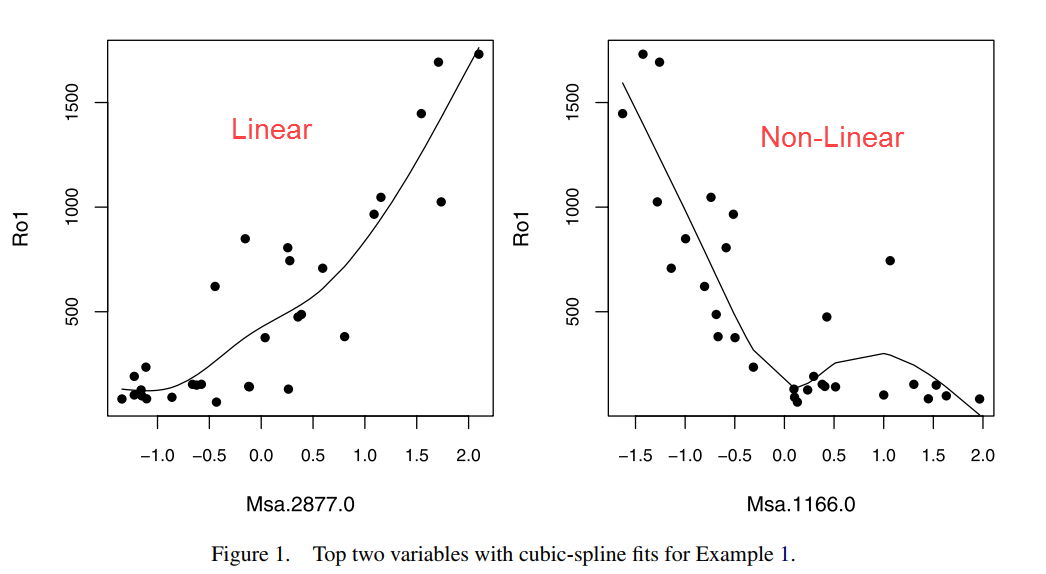
\includegraphics[width=0.70000\textwidth]{./figure/overlooking.png}

\begin{itemize}
\tightlist
\item
  Micoroarray data of heart disease\\
\item
  Ro1: expression level, continuous response\\
\item
  Msa: different genes, continuous predictor
\end{itemize}

\end{frame}

\begin{frame}{The Collinearity}

\begin{itemize}
\tightlist
\item
  Even the model is perfectly linear, fitting a linear model may conceal
  importance components of X just because of the collinearity
\item
  It's also called the ``masking effect'', which means we only can
  select part of the important variables
\item
  However, at point of variable selection, we want to be able to select
  all of them
\item
  Back to the previous heat disease example,
  \(cor(Msa.2877, Msa.1166) = -0.71\). So it's possible that the
  collinearity prevents us to find the Msa.1166
\end{itemize}

\end{frame}

\section{Solution: Generalized
Correlation}\label{solution-generalized-correlation}

\begin{frame}{Generalized Correlation}

\begin{block}{Generalized Correlation coefficient between $X_{ij}$ and $Y_i$}

\[
  \sup\limits_{h \in \mathcal{H}} \frac{cov\{h(X_{ij}), Y_i\}}{\sqrt{var\{h(X_{ij})\}, var(Y_i)}}
\]
Estimated by,
\[
\sup\limits_{h \in \mathcal{H}} \frac{\sum_i\{h(X_{ij}) - \bar{h}\}(Y_i - \bar{Y})}{\sqrt{\sum_i {\{h(X_{ij})-\bar{h}\}}^2 \cdot \sum_i {(Y_i - \bar{Y})}^2}}
\]
\end{block}

\begin{itemize}
\tightlist
\item
  \((X_1, Y_1), \dots, (X_n, Y_n)\) are iid
\item
  X is p-vectors
\item
  Y is scalars
\item
  \(\mathcal{H}\) is a vector space of functions
\item
  \(\bar{h} = n^{-1}\sum_ih(X_{ij})\)
\end{itemize}

\end{frame}

\begin{frame}{Simplify the computation}

\begin{block}{Removing $Var(Y_i)$}
    \begin{align*} 
      \psi_j &= \sup\limits_{h \in \mathcal{H}} \frac{cov\{h(X_{ij}), Y_i\}}{\sqrt{var\{h(X_{ij})\}}} \\   
      \hat{\psi}_j &= \sup\limits_{h \in \mathcal{H}} \frac{\sum_i\{h(X_{ij}) - \bar{h}\}(Y_i - \bar{Y})}{\sqrt{n\sum_i \{h(X_{ij})-\bar{h}\}^2}}
    \end{align*} 
\end{block}

\begin{itemize}
\tightlist
\item
  Since \(Var(Y_i)\) is same for each i, we can remove it without
  affecting the ranking of the correlation
\end{itemize}

\end{frame}

\begin{frame}{Simplify the computation Cont.}

\begin{block}{Theorem 1}
Assume $\mathcal{H}$ is a finite-dimensional function space include the constant function, and there exists $ h\in\mathcal{H}$ that achieves $\hat{\psi}_j$,

\[
\argmin{h \in \mathcal{H}} \sum^n\limits_{i = 1}\{Y_i - h(X_{ij})\}^2 \subseteq \argmax{h \in \mathcal{H}} \hat{\psi}_j
\]
The maximizer of $\hat{\psi}_j$ is the solution to least squares problem in $\mathcal{H}$
\end{block}

\begin{block}{Reduction of $\hat{\psi}_j$ in the size of squared error}
\[
  \hat{\varphi}_j = \sum^n\limits_{i = 1} (Y_i - \hat{Y})^2 - \inf\limits_{h \in \mathcal{H}}\sum^n\limits_{i = 1}\{Y_i - h(X_{ij})\}^2
\]
Since $\hat{\varphi}_j$ keeps the relative relation of $\hat{\psi}_j$, we can use $\hat{\varphi}_j$'s for ranking
\end{block}

\end{frame}

\begin{frame}{Correlation Ranking}

\begin{block}{Some notations}

\begin{itemize}
\item
  We order estimator \(\hat{\psi}_j\) as
  \(\hat{\psi}_{\hat{j}_1} \geq \dots \geq \hat{\psi}_{\hat{j}_p}\) \[
    \hat{j}_1 \succeq \dots \succeq \hat{j}_p
  \]
\item
  \(j \succeq j'\) means \(\hat{\psi}_j \geq \hat{\psi}_{j'}\), we could
  say jth coefficient of X is at least as much importance as the j'th
  coefficient
\item
  \(r = \hat{r}(j)\) means the rank of the jth coefficient is r, in
  other words \(\hat{j}_r = j\)
\end{itemize}

\end{block}

\end{frame}

\begin{frame}{Estimation of the rank}

We could use Bootstrap to assess the empirical rank for each component
of X\\
A \((1-\alpha)\) level, two-side interval is defined as following:

\begin{block}{Interval of rank $[\hat{r}_{-}(j), \hat{r}_{+}(j)]$}
\[
  P\{r^*(j)\leq \hat{r}_{-}(j)|\mathcal{D}\} \approx P\{r^*(j)\geq \hat{r}_{+}(j)|\mathcal{D}\} \approx \frac{\alpha}{2}
\]
\end{block}

\begin{itemize}
\tightlist
\item
  \(r^*(j)\) the bootstrap version estimators of \(r(j)\)
\item
  The approximation is used because of the discreteness of ranks
\item
  Small value of \(r^*(j)\) indicates large influence on Y
\item
  In order to select variables, we could sort \(r^*(j)\) or
  \(\hat{r}_{+}(j)\) and set a cut off value \(p\)
\end{itemize}

\end{frame}

\section{Simulation study}\label{simulation-study}

\begin{frame}{heart disease data}

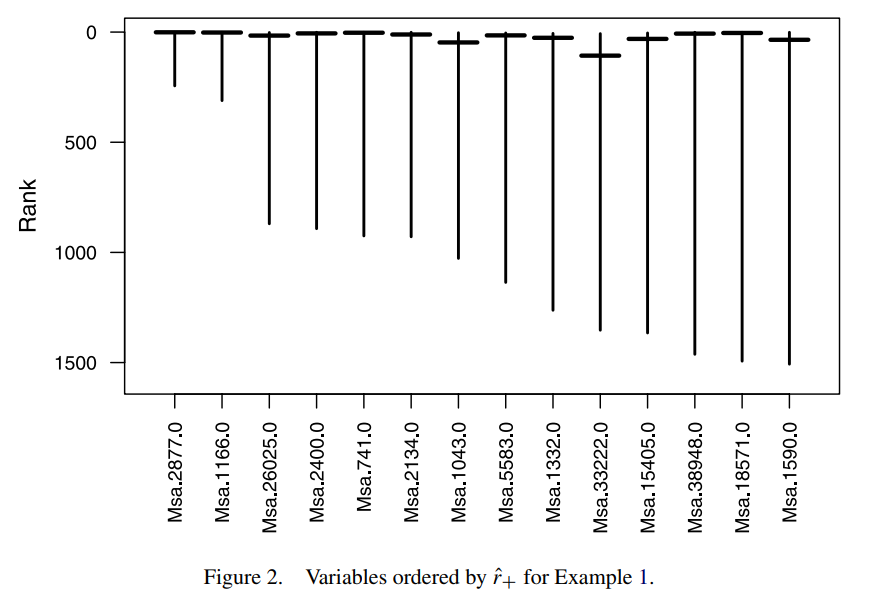
\includegraphics[width=0.70000\textwidth]{./figure/rank_heart_diseas.png}

\begin{itemize}
\tightlist
\item
  \(n =30\), \(p = 6319\)
\item
  bootstrap sample is 400
\item
  \(\alpha = 0.02\) cutoff value is \(p/4\)
\item
  ranking is based on \(\hat{r}_{+}(j)\)
\item
  Note: There is a marked jump in the length of the predict intervals
\end{itemize}

\end{frame}

\begin{frame}{Simulation study on non-linear model}

\begin{block}{simulation setup} 
\[
  Y_i = W^2_i -1 + \epsilon_i
\]
\end{block}

\begin{itemize}
\tightlist
\item
  \(W_i \sim Unif[-2,2]\)
\item
  \(X_{i1} = W_{i} + \delta_i\) (errors-in-variables type)
\item
  \(X_{i2}, \dots, X_{i5000} \stackrel{iid}{\sim} N(0,1)\)
\item
  \(\delta, \epsilon \stackrel{iid}{\sim} N(0, 3/4)\)
\item
  \(n = 200, ~ \alpha = 0.02, n_{bootstrap} = 500\)
\end{itemize}

\end{frame}

\begin{frame}{Simulation study on non-linear model Cont.}

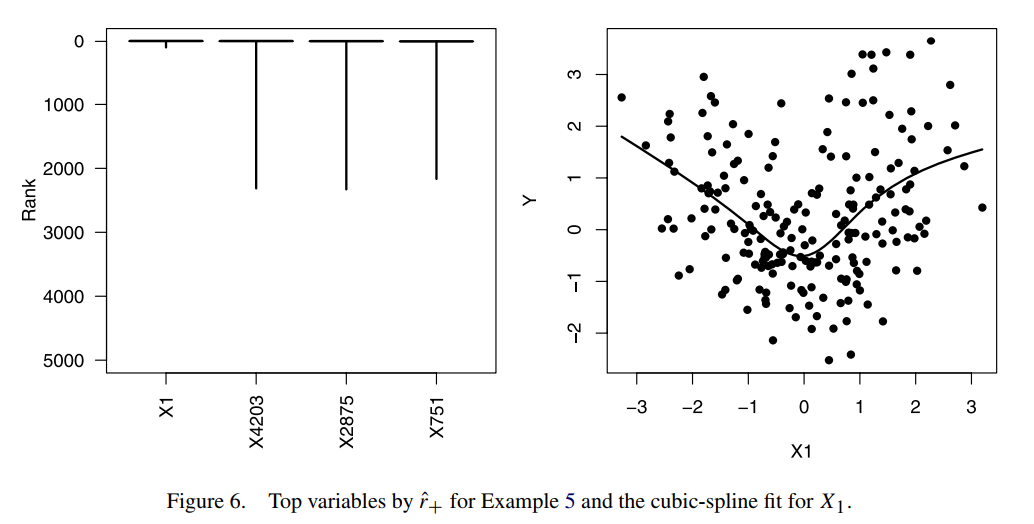
\includegraphics[width=0.70000\textwidth]{./figure/sim_non_linear.png}

\begin{itemize}
\tightlist
\item
  the cutoff value is \(p/2\)\\
\item
  Conventional correlation fails to select \(X_{i1}\) as influential
  variable\\
\item
  Generalized correlation method is able to select the \(X_{i1}\) with
  only 3 false positive variables
\end{itemize}

\end{frame}

\section{Conclusion}\label{conclusion}

\begin{frame}{Potential applications}

\begin{itemize}
\tightlist
\item
  It can be used as a ``massive dimension reduction'' method
\item
  It should be a more effective variable selection method for
  (Generalized) Additive Model
\end{itemize}

\end{frame}

\begin{frame}{Further topics}

\begin{itemize}
\tightlist
\item
  Unbiasedness and Consistency of the selected Variables\\
\item
  The choice of cutoff value
\end{itemize}

\end{frame}

\begin{frame}{}

\begin{center}
\Huge Thank you
\end{center}

\end{frame}

\begin{frame}{Reference}

\hypertarget{refs}{}
\hypertarget{ref-ref6}{}
Peter HALL, Hugh MILLER. 2009. ``Using Generalized Correlation to Effect
Variable Selection in Very High Dimensional Problems.''

\end{frame}

\end{document}
